\documentclass[aspectratio=169,11pt]{beamer}
\usepackage[T1]{fontenc}
\usepackage[utf8]{inputenc}
\usepackage[spanish]{babel}
\usepackage{lmodern}
\usepackage{amsmath,amssymb,mathtools}
\usepackage{xcolor}
\usepackage{graphicx}
\usepackage{array}
\usepackage{tikz}
\usetikzlibrary{calc,positioning}
\usepackage{hyperref}

\definecolor{UdeAGreen}{HTML}{0D6939}
\definecolor{DeepGreen}{HTML}{064629}
\definecolor{LeafGreen}{HTML}{83B840}
\definecolor{PaleGreen}{HTML}{E7F0E7}
\definecolor{CardGreen}{HTML}{F5F8F3}
\definecolor{Ink}{HTML}{173629}
\definecolor{WarmGold}{HTML}{E5C45A}
\definecolor{SoftGray}{HTML}{68766E}

\usetheme{Boadilla}
\setbeamertemplate{navigation symbols}{}
\setbeamertemplate{blocks}[rounded][shadow=false]
\setbeamercolor{normal text}{fg=Ink,bg=PaleGreen}
\setbeamercolor{background canvas}{bg=PaleGreen}
\setbeamercolor{structure}{fg=UdeAGreen}
\setbeamercolor{frametitle}{fg=white,bg=DeepGreen}
\setbeamerfont{frametitle}{series=\bfseries,size=\large}
\setbeamercolor{title}{fg=white}
\setbeamercolor{subtitle}{fg=white!85}
\setbeamercolor{block title}{fg=white,bg=UdeAGreen}
\setbeamercolor{block body}{fg=Ink,bg=CardGreen}
\setbeamercolor{block title example}{fg=DeepGreen,bg=LeafGreen!55}
\setbeamercolor{block body example}{fg=Ink,bg=CardGreen}
\setbeamercolor{block title alerted}{fg=white,bg=DeepGreen}
\setbeamercolor{block body alerted}{fg=Ink,bg=CardGreen}
\setbeamercolor{author in head/foot}{fg=white,bg=DeepGreen}
\setbeamertemplate{footline}{%
  \leavevmode%
  \hbox{\begin{beamercolorbox}[wd=\paperwidth,ht=2.6ex,dp=1.1ex,leftskip=1em,rightskip=1em]{author in head/foot}%
  Introducción al grupo\hfill Grupo de Estudio · UdeA\hfill\insertframenumber/\inserttotalframenumber
  \end{beamercolorbox}}%
}
\setbeamertemplate{itemize item}{\color{UdeAGreen}\small$\blacktriangleright$}
\setbeamertemplate{itemize subitem}{\color{LeafGreen}\scriptsize$\blacktriangleright$}
\setbeamertemplate{enumerate items}[circle]
\setbeamercolor{item projected}{fg=white,bg=UdeAGreen}
\setlength{\leftmargini}{1.5em}

\newcommand{\NN}{\mathbb{N}}
\newcommand{\ZZ}{\mathbb{Z}}
\newcommand{\QQ}{\mathbb{Q}}
\newcommand{\RR}{\mathbb{R}}
\newcommand{\CC}{\mathbb{C}}
\newcommand{\units}[1]{(\mathbb{Z}/#1\mathbb{Z})^{\times}}
\newcommand{\Set}[1]{\left\{#1\right\}}

\title[Introducción al grupo]{Grupo de Estudio de Teoría Analítica de Números}
\subtitle{De los fundamentos a las funciones L de Dirichlet}
\author{Daniel Soto Villada}
\institute{Facultad de Ciencias Exactas y Naturales · Universidad de Antioquia}
\date{12 de noviembre de 2026}

\begin{document}

{\setbeamercolor{background canvas}{bg=DeepGreen}
\begin{frame}[plain]
    \begin{tikzpicture}[remember picture,overlay]
        \node[anchor=center] at ([xshift=-2.5cm]current page.east)
            {
\includegraphics[width=7.5cm]{LogoUdeA_Blanco.png}};
    \end{tikzpicture}
    \vspace{0.65cm}
    {\color{WarmGold}\bfseries\large UNIVERSIDAD DE ANTIOQUIA}\par
    \vspace{0.48cm}
    {\color{white}\bfseries\fontsize{29}{34}\selectfont TEORÍA ANALÍTICA\\DE NÚMEROS}\par
    \vspace{0.25cm}
    {\color{white!85}\Large Presentación del grupo de estudio}\par
    \vspace{1.05cm}
    {\color{white}\large Daniel Soto Villada}\par
    \vspace{0.15cm}
    {\color{white!80}\normalsize Facultad de Ciencias Exactas y Naturales}\par
    \vfill
    {\color{LeafGreen}\large Jueves 12 de noviembre de 2026\hspace{1em}$\cdot$\hspace{1em}Aula 4-218}\par
    \vspace{0.45cm}
\end{frame}}

\begin{frame}{¿Qué es este grupo de estudio?}
    \begin{block}{Propósito}
        Construir de manera gradual las herramientas matemáticas que permiten formular y comprender preguntas de teoría analítica de números.
    \end{block}
    \begin{itemize}
        \item No partimos suponiendo que ya se conoce análisis complejo o álgebra abstracta.
        \item Avanzaremos desde los fundamentos, haciendo explícitas las definiciones y las demostraciones.
        \item Cada tema prepara el lenguaje y las técnicas de los siguientes.
        \item El objetivo es entender ideas y argumentos, no memorizar fórmulas aisladas.
    \end{itemize}
\end{frame}

\begin{frame}{¿A quién está dirigido y cómo participamos?}
    \begin{columns}[T,onlytextwidth]
        \column{.48\textwidth}
        \begin{block}{Dirigido a}
            Estudiantes de pregrado con interés por las matemáticas y sus conexiones.
            \begin{itemize}
                \item Prerrequisito: matemáticas básicas.
                \item No se requiere inscripción previa.
            \end{itemize}
        \end{block}
        \column{.48\textwidth}
        \begin{exampleblock}{Encuentros}
            \begin{itemize}
                \item Todos los jueves.
                \item 14:00--16:00.
                \item Aula 4-218.
                \item Facultad de Ciencias Exactas y Naturales, Universidad de Antioquia.
            \end{itemize}
        \end{exampleblock}
    \end{columns}
\end{frame}

\begin{frame}{La pregunta que nos convoca: ¿cómo se distribuyen los primos?}
    Los números primos comienzan así:
    \[
      2,\;3,\;5,\;7,\;11,\;13,\;17,\;19,\;23,\;29,\ldots
    \]
    \begin{itemize}
        \item ¿Cuántos primos hay por debajo de un número grande $x$?
        \item ¿Aparecen con frecuencia regular o irregular?
        \item ¿Cómo se distribuyen entre las clases de residuos?
    \end{itemize}
    \begin{block}{Función de conteo}
        $\pi(x)=\#\{p\leq x:p\text{ es primo}\}$ cuenta los primos que no exceden $x$.
    \end{block}
    \centering\small Estas preguntas conectan la aritmética de los enteros con herramientas de análisis.\;\cite[Capítulos 1--2]{Apostol1976-xj}
\end{frame}

\begin{frame}{¿Qué significa «analítica» en teoría de números?}
    \begin{block}{Idea general}
        La teoría analítica de números estudia propiedades de los enteros —en especial, de los primos— usando herramientas del análisis matemático.
    \end{block}
    \begin{columns}[T,onlytextwidth]
        \column{.48\textwidth}
        \textbf{Objetos aritméticos}
        \begin{itemize}
            \item primos y divisibilidad;
            \item congruencias y residuos;
            \item funciones que cuentan o ponderan enteros.
        \end{itemize}
        \column{.48\textwidth}
        \textbf{Herramientas analíticas}
        \begin{itemize}
            \item sucesiones y series infinitas;
            \item funciones de variable compleja;
            \item límites, integrales y estimaciones.
        \end{itemize}
    \end{columns}
    \vfill
    \centering\small Una serie puede convertir una pregunta sobre enteros en una pregunta sobre una función.
\end{frame}

\begin{frame}{Una primera imagen de la distribución de los primos}
    \centering
    \begin{tikzpicture}[x=.34cm,y=.30cm]
        \foreach \x in {5,10,...,30} {
            \draw[gray!22,thin] (\x,0) -- (\x,12);
            \draw[black] (\x,0) -- (\x,-.35);
            \node[below=3pt,font=\scriptsize] at (\x,0) {$\x$};
        }
        \foreach \y in {2,4,...,12} {
            \draw[gray!22,thin] (0,\y) -- (32,\y);
            \draw[black] (0,\y) -- (-.5,\y);
            \node[left=3pt,font=\scriptsize] at (0,\y) {$\y$};
        }
        \draw[->,thick] (0,0) -- (33,0) node[below right] {$x$};
        \draw[->,thick] (0,0) -- (0,12.7) node[above left] {$\pi(x)$};
        \draw[blue!70!black,very thick]
            (0,0)--(2,0)--(2,1)--(3,1)--(3,2)--(5,2)--(5,3)
            --(7,3)--(7,4)--(11,4)--(11,5)--(13,5)--(13,6)
            --(17,6)--(17,7)--(19,7)--(19,8)--(23,8)--(23,9)
            --(29,9)--(29,10)--(32,10);
        \draw[orange!85!black,very thick,samples=120,domain=2:30,smooth,variable=\t]
            plot (\t,{\t/ln(\t)});
        \node[blue!70!black,anchor=west,font=\small] at (32,10) {$\pi(x)$};
        \node[orange!85!black,anchor=west,font=\small] at (30.4,8.4) {$x/\log x$};
    \end{tikzpicture}

    \vspace{-.1cm}
    \small La gráfica sugiere la aproximación $\pi(x)\sim x/\log x$ cuando $x$ crece; no constituye por sí sola una demostración.\;\cite[Capítulo 4]{Apostol1976-xj}
\end{frame}

\begin{frame}{Un recorrido histórico en cuatro retratos}
    La teoría analítica de números se construyó a lo largo de generaciones:
    \begin{itemize}
        \item \textbf{Euler:} conecta una suma sobre enteros con un producto sobre primos.
        \item \textbf{Dirichlet:} usa series para demostrar que hay infinitos primos en progresiones aritméticas admisibles.
        \item \textbf{Riemann:} relaciona la función zeta compleja con la distribución de los primos.
        \item \textbf{Ramanujan:} desarrolla ideas profundas sobre particiones, series y funciones aritméticas.
    \end{itemize}
\end{frame}

\begin{frame}{Leonhard Euler (1707--1783): primos e infinitos productos}
    \begin{columns}[T,onlytextwidth]
        \column{.32\textwidth}
        \centering
        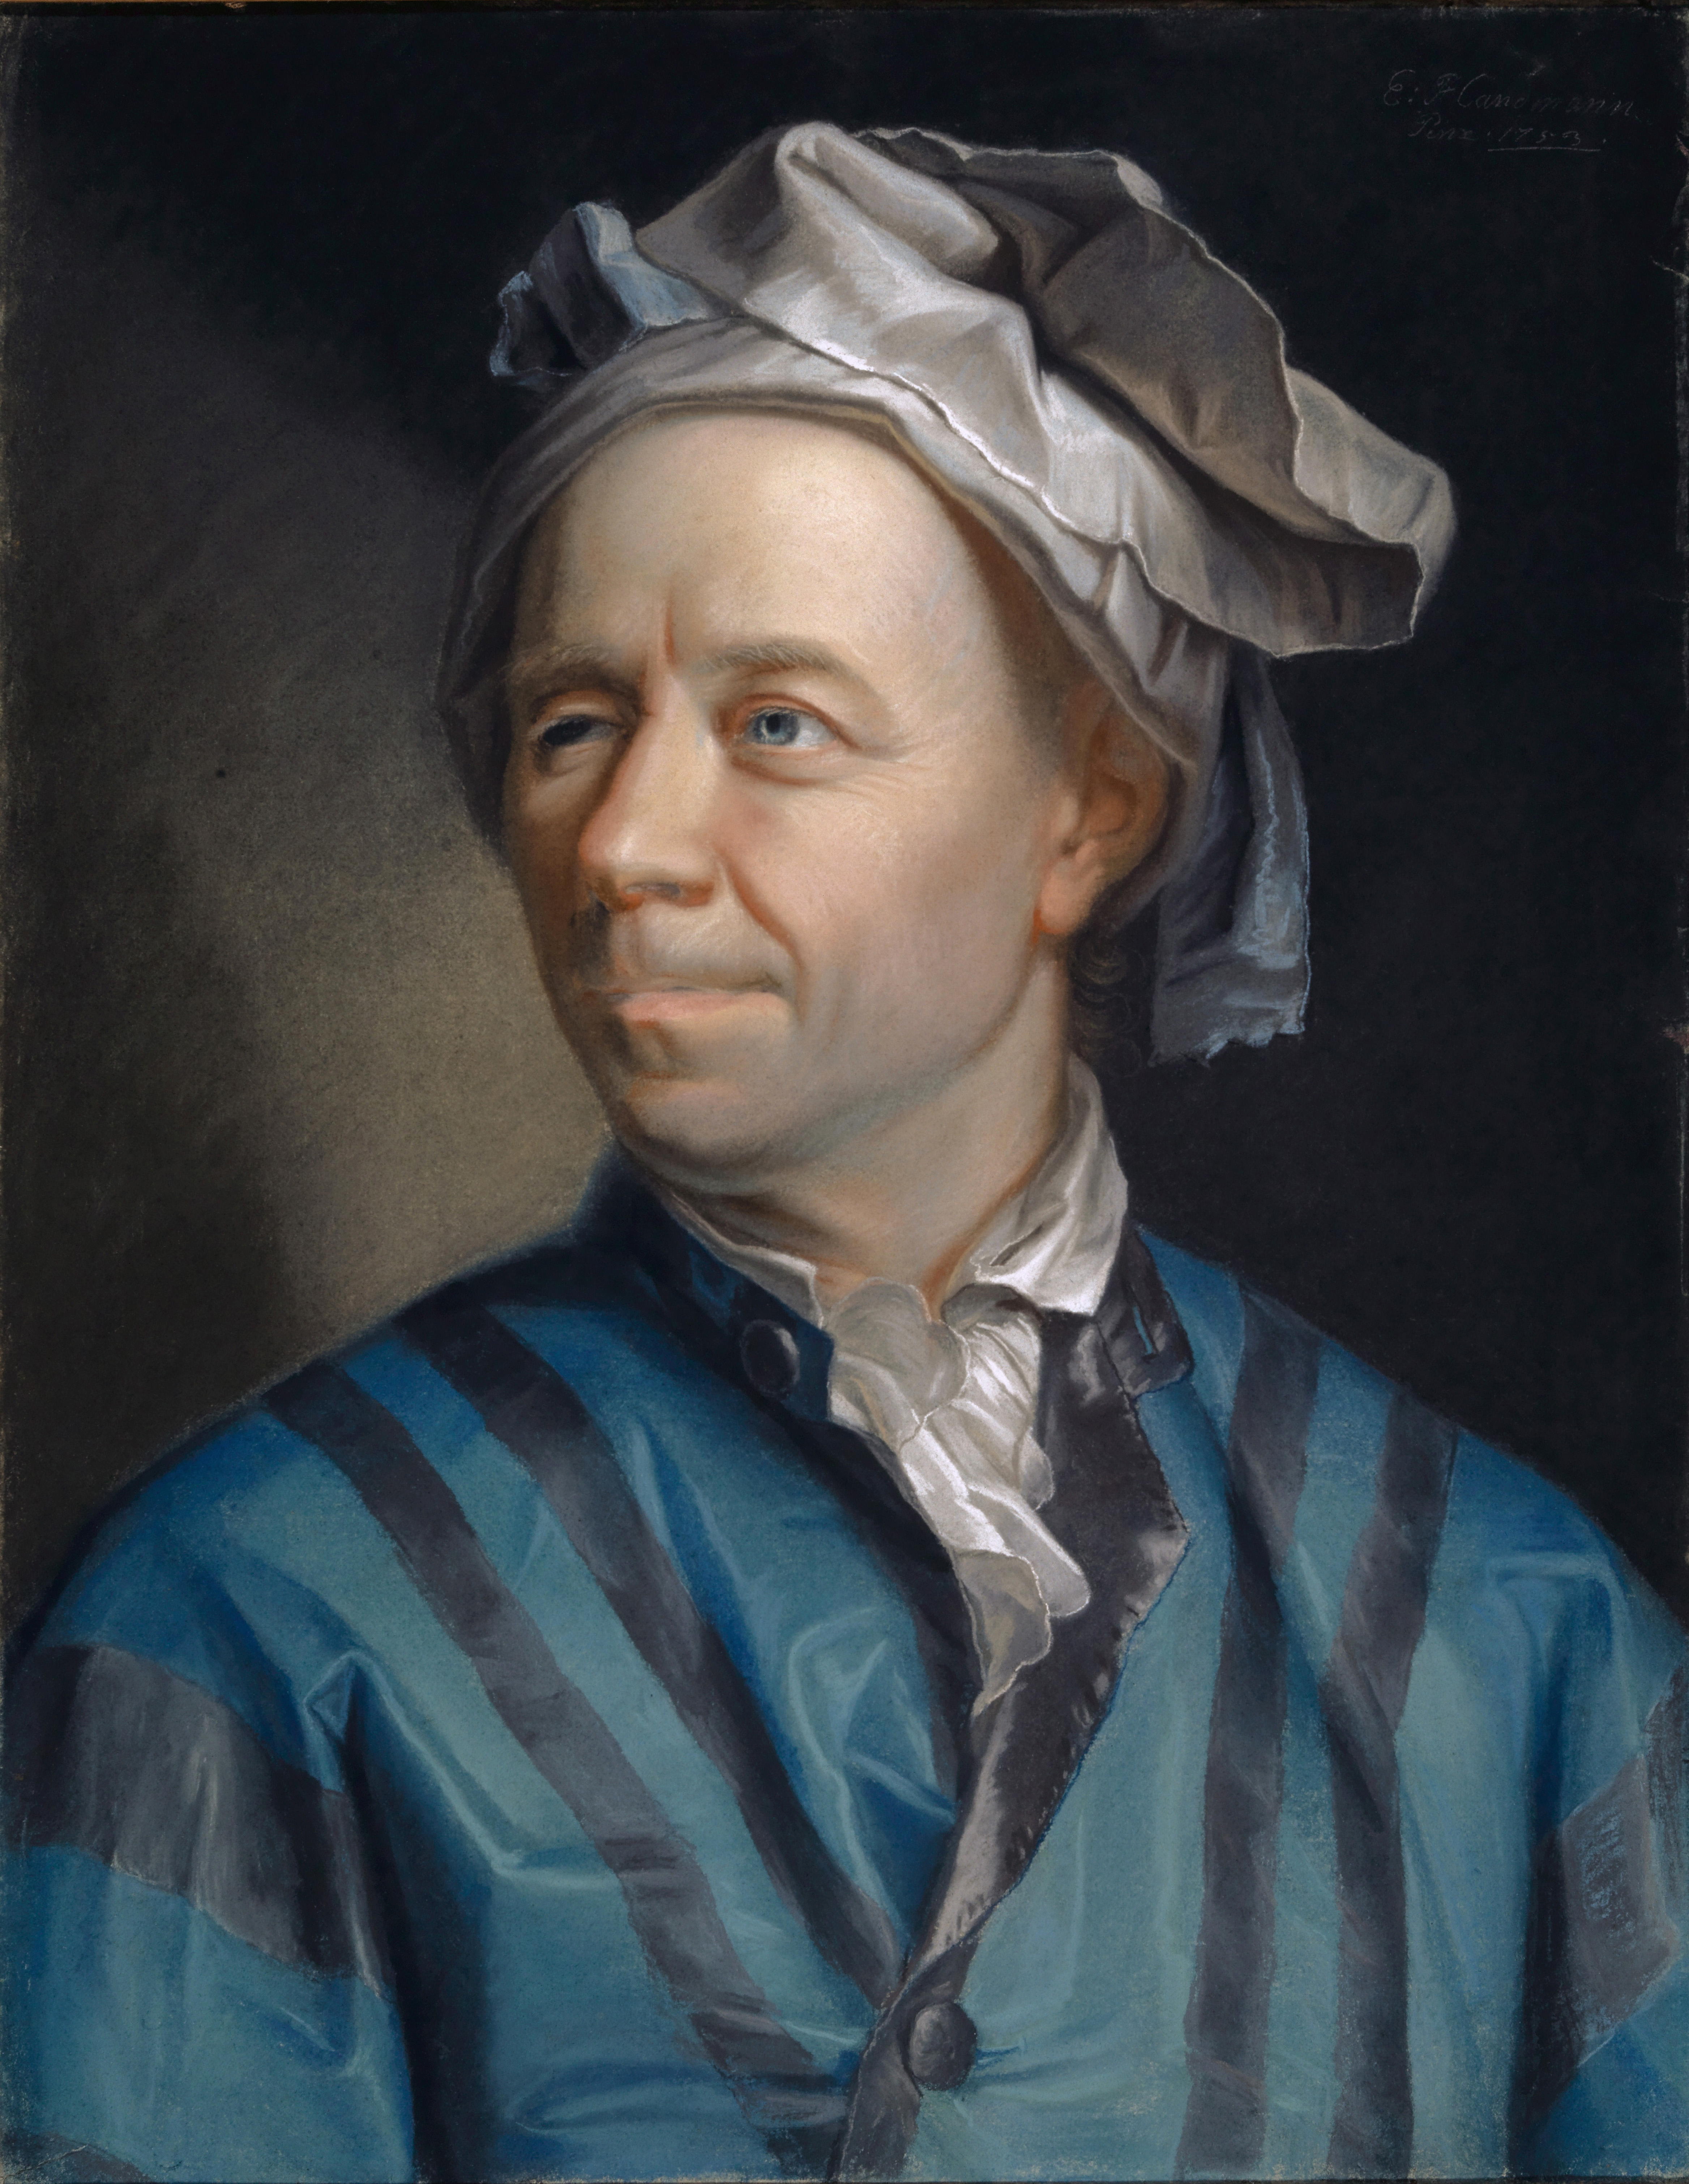
\includegraphics[height=.62\textheight,keepaspectratio]{FigurasClase0/Euler.jpg}
    \column{.64\textwidth}
        Euler obtuvo una conexión fundamental entre la serie sobre todos los enteros positivos y el producto sobre los primos:
        \[
          \sum_{n=1}^{\infty}\frac{1}{n^s}
          =\prod_p\left(1-p^{-s}\right)^{-1},
          \qquad s>1.
        \]
        \begin{itemize}
            \item La factorización única de los enteros explica por qué aparecen los primos en el producto.
            \item Esta identidad es el modelo de los productos de Euler que aparecerán para las funciones $L$.
            \item El resultado suele fecharse en 1737; la formulación moderna se estudia en su región de convergencia.
        \end{itemize}
        {\footnotesize\cite{Apostol1976-xj}}
    \end{columns}
\end{frame}

\begin{frame}{Johann Peter Gustav Lejeune Dirichlet (1805--1859)}
    \begin{columns}[T,onlytextwidth]
        \column{.32\textwidth}
        \centering
        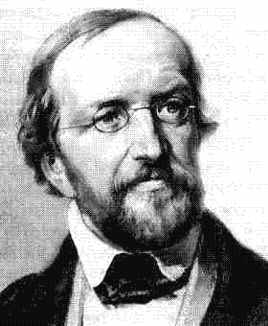
\includegraphics[height=.62\textheight,keepaspectratio]{FigurasClase0/Dirichlet.jpg}
    \column{.64\textwidth}
        En 1837 demostró un resultado que abre una nueva perspectiva sobre los primos:
        \begin{block}{Teorema de Dirichlet}
            Si $\gcd(a,k)=1$, la progresión
            \[
              a,\;a+k,\;a+2k,\;a+3k,\ldots
            \]
            contiene infinitos números primos.
        \end{block}
        \begin{itemize}
            \item Su demostración introduce series de Dirichlet y herramientas que anticipan los caracteres.
            \item Por ejemplo, hay infinitos primos congruentes con $1$ módulo $4$ y también con $3$ módulo $4$.
        \end{itemize}
        {\footnotesize\cite{Apostol1976-xj}}
    \end{columns}
\end{frame}

\begin{frame}{Bernhard Riemann (1826--1866): una función compleja para contar primos}
    \begin{columns}[T,onlytextwidth]
        \column{.32\textwidth}
        \centering
        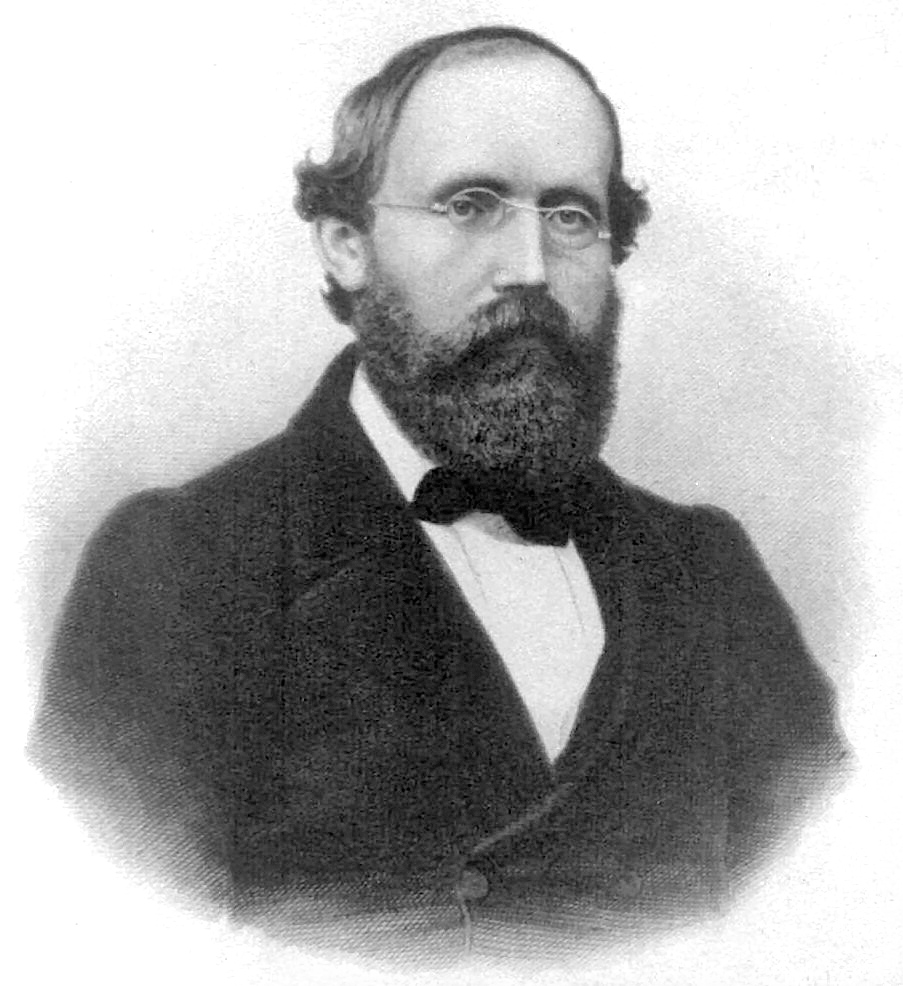
\includegraphics[height=.62\textheight,keepaspectratio]{FigurasClase0/Riemann.jpeg}
    \column{.64\textwidth}
        En su memoria de 1859 sobre los primos menores que una magnitud dada, Riemann estudió la zeta como función de una variable compleja:
        \[
          \zeta(s)=\sum_{n=1}^{\infty}\frac{1}{n^s}
          =\prod_p(1-p^{-s})^{-1},\qquad \Re(s)>1.
        \]
        \begin{itemize}
            \item Relacionó los ceros de la zeta con las oscilaciones en el conteo de primos.
            \item Planteó que los ceros no triviales estarían en $\Re(s)=\tfrac12$.
            \item Esta conjetura, la Hipótesis de Riemann, sigue abierta.
        \end{itemize}
        {\footnotesize\cite{Apostol1976-xj,Broughan2017}}
    \end{columns}
\end{frame}

\begin{frame}{Srinivasa Ramanujan (1887--1920): patrones aritméticos inesperados}
    \begin{columns}[T,onlytextwidth]
        \column{.32\textwidth}
        \centering
        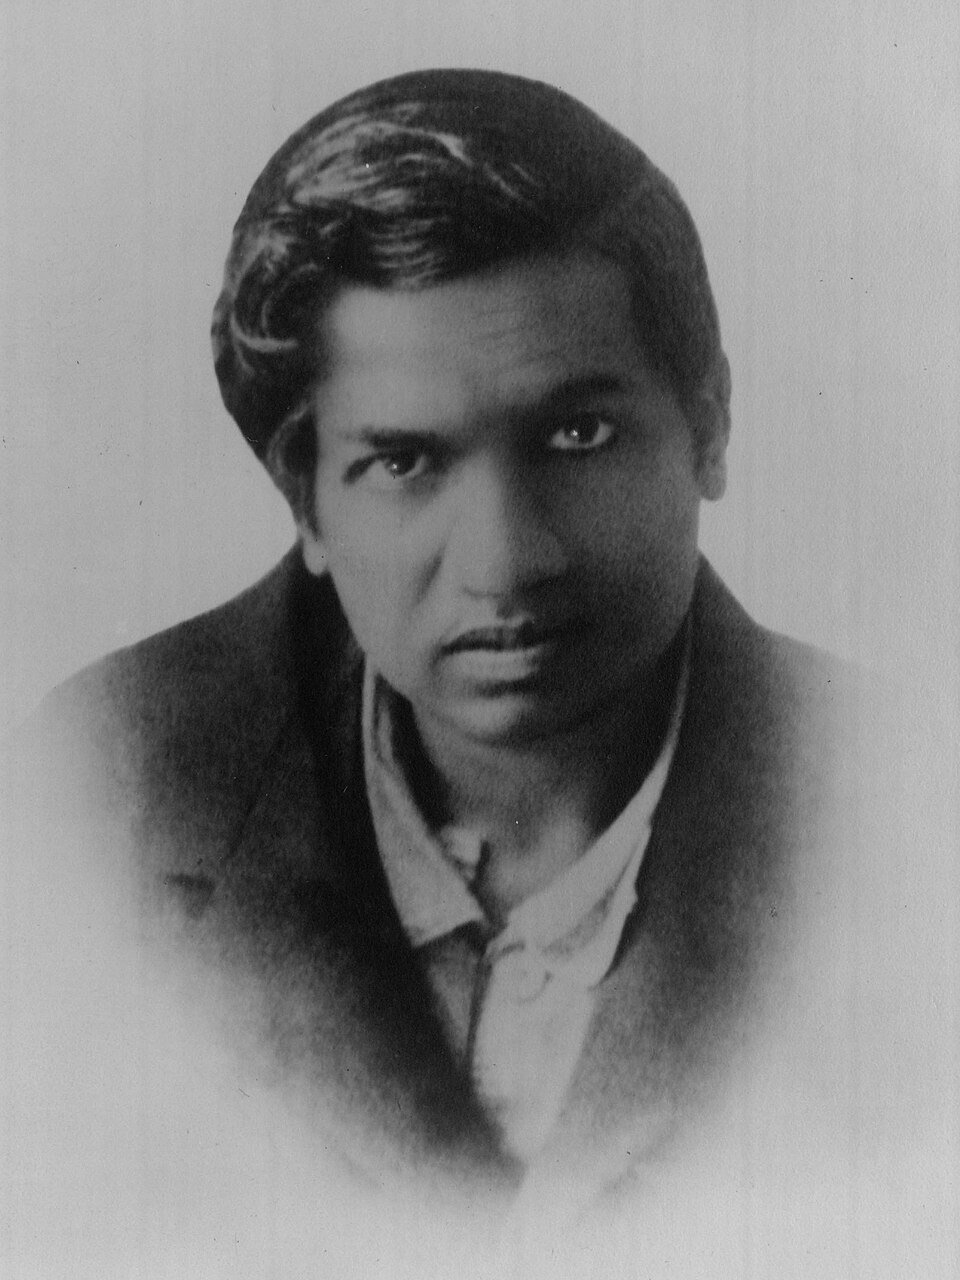
\includegraphics[height=.62\textheight,keepaspectratio]{FigurasClase0/Ramanujan.jpg}
    \column{.64\textwidth}
        Ramanujan investigó series infinitas, funciones elípticas y particiones de enteros.
        \begin{block}{Congruencia de Ramanujan}
            Sea $p(n)$ el número de particiones de $n$ en sumas de enteros positivos. Entonces
            \[
              p(5m+4)\equiv0\pmod 5,\qquad m\geq0.
            \]
        \end{block}

    \end{columns}
\end{frame}


\section{\texorpdfstring{La función $L$ aparece antes que su carácter}{La función L aparece antes que su carácter}}
\begin{frame}{Primero, la función $L$ de Dirichlet}
    Para un módulo $k\geq2$ y una función $\chi$ adecuada, consideremos
    \[
      \boxed{L(s,\chi)=\sum_{n=1}^{\infty}\frac{\chi(n)}{n^s}},
      \qquad \Re(s)>1.
    \]
    Si $\chi$ es multiplicativa, la serie también tiene un producto sobre los primos:
    \[
      L(s,\chi)=\prod_p\left(1-\frac{\chi(p)}{p^s}\right)^{-1}.
    \]
    \begin{itemize}
        \item La suma recorre los enteros positivos.
        \item El producto recorre los primos.
        \item Los valores $\chi(n)$ ponderan los términos según la aritmética módulo $k$.
    \end{itemize}
    \centering\small La definición y el producto se justifican en el semiplano de convergencia absoluta $\Re(s)>1$.\;\cite[Capítulos 6--7]{Apostol1976-xj}
\end{frame}

\begin{frame}{La pregunta natural: ¿qué es el carácter $\chi$?}
    En la serie
    \[
      L(s,\chi)=\frac{\chi(1)}{1^s}+\frac{\chi(2)}{2^s}+\frac{\chi(3)}{3^s}+\cdots,
    \]
    ¿qué regla determina los coeficientes $\chi(1),\chi(2),\chi(3),\ldots$?
    \begin{exampleblock}{Pistas que debe cumplir}
        La regla debe reconocer residuos módulo $k$, repetirse periódicamente y respetar la multiplicación de enteros.
    \end{exampleblock}
    \begin{alertblock}{La dificultad pedagógica}
        Para entender la palabra «carácter» necesitamos primero conjuntos de residuos, unidades módulo $k$, grupos y homomorfismos; después, para entender $L(s,\chi)$, necesitamos series y análisis complejo.
    \end{alertblock}
    \centering\color{UdeAGreen}\bfseries Vamos a construir esas ideas en el orden necesario.
\end{frame}

\begin{frame}{Una primera muestra: el carácter módulo $4$}
    Una función que distingue las dos clases impares módulo $4$ es
    \[
      \chi_4(n)=
      \begin{cases}
        0,&n\text{ es par},\\
        1,&n\equiv1\pmod4,\\
        -1,&n\equiv3\pmod4.
      \end{cases}
    \]
    Por tanto,
    \[
      L(s,\chi_4)=1-\frac{1}{3^s}+\frac{1}{5^s}-\frac{1}{7^s}+\cdots.
    \]
    \begin{itemize}
        \item Periodicidad: los valores se repiten cada cuatro enteros.
        \item Multiplicatividad: $\chi_4(mn)=\chi_4(m)\chi_4(n)$.
        \item Los pares reciben valor cero porque no son coprimos con $4$.
    \end{itemize}
    \centering\small Más adelante probaremos estas propiedades a partir de la estructura de las unidades módulo $4$.
\end{frame}

\begin{frame}{El mapa de dependencias: del entero a la función $L$}
    \centering
    \begin{tikzpicture}[node distance=1.05cm,every node/.style={align=center}]
        \node[draw=UdeAGreen,fill=CardGreen,rounded corners,inner sep=5pt,text width=2.2cm] (arithmetic) {Enteros, primos y\\congruencias};
        \node[draw=UdeAGreen,fill=CardGreen,rounded corners,inner sep=5pt,text width=2.2cm,right=of arithmetic] (units) {Clases y grupo\\de unidades};
        \node[draw=UdeAGreen,fill=CardGreen,rounded corners,inner sep=5pt,text width=2.2cm,font=\scriptsize,right=of units] (character) {Homomorfismos\\y caracteres};
        \node[draw=UdeAGreen,fill=CardGreen,rounded corners,inner sep=5pt,text width=2.2cm,right=of character] (L) {Series\\$L(s,\chi)$};
        \draw[->,thick,LeafGreen!80!black] (arithmetic)--(units);
        \draw[->,thick,LeafGreen!80!black] (units)--(character);
        \draw[->,thick,LeafGreen!80!black] (character)--(L);
    \end{tikzpicture}
    \vspace{.7cm}
    \begin{block}{En paralelo}
        Análisis real aporta convergencia; análisis complejo aporta continuación analítica, polos, ceros y ecuaciones funcionales.
    \end{block}
\end{frame}

\section{Los prerrequisitos matemáticos}
\begin{frame}{Sección I: conjuntos, relaciones y funciones}
    \begin{itemize}
        \item Escribir conjuntos por extensión y por comprensión.
        \item Distinguir pertenencia $x\in A$ de inclusión $A\subseteq B$.
        \item Trabajar con pares ordenados y productos cartesianos.
        \item Entender relaciones, equivalencias, clases de residuos y funciones.
    \end{itemize}
    \begin{exampleblock}{Por qué son necesarios}
        Una congruencia es una relación de equivalencia; sus clases forman $\mathbb{Z}/k\mathbb{Z}$, y de allí se construye el grupo de unidades.
    \end{exampleblock}
\end{frame}

\begin{frame}{Sección II: divisibilidad, primos y máximo común divisor}
    Para $a,b\in\ZZ$, $a\mid b$ significa que $b=aq$ para algún $q\in\ZZ$.
    \begin{itemize}
        \item Primos: enteros positivos mayores que $1$ con solo dos divisores positivos.
        \item $\gcd(a,b)$: el mayor divisor común positivo.
        \item Coprimalidad: $\gcd(a,k)=1$.
        \item Teorema fundamental de la aritmética: factorización única en primos.
    \end{itemize}
    \begin{exampleblock}{Cálculo breve}
        $\gcd(18,35)=1$; por ello, $18$ es invertible módulo $35$ y es admisible como primer término de una progresión de primos con diferencia $35$.
    \end{exampleblock}
    \centering\small Divisibilidad y factorización son el vocabulario aritmético básico.\;\cite[Capítulo 1]{Apostol1976-xj}
\end{frame}

\begin{frame}{Sección III: congruencias y clases de residuos}
    Para $a,b\in\ZZ$ y $k\in\ZZ$, con $k\geq2$,
    \[
      a\equiv b\pmod k\quad\Longleftrightarrow\quad k\mid(a-b).
    \]
    \begin{block}{Forma general de una clase y del conjunto cociente}
        \[
          [a]_k=\{b\in\ZZ:b\equiv a\pmod k\}
              =\{a+qk:q\in\ZZ\},\qquad
          \ZZ/k\ZZ=\{[0]_k,[1]_k,\ldots,[k-1]_k\}.
        \]
    \end{block}
    \begin{exampleblock}{Ejemplo: módulo $5$}
        \[
          [2]_5=\{\ldots,-8,-3,2,7,12,\ldots\},
          \qquad 17\in[2]_5.
        \]
    \end{exampleblock}
    \small Las clases particionan $\ZZ$; la suma y el producto módulo $k$ se definen sobre ellas.
\end{frame}

\begin{frame}{Sección IV: unidades y función totiente}
    En $\ZZ/k\ZZ$, no todas las clases tienen inverso multiplicativo. Las invertibles forman el grupo
    \begin{block}{Grupo de unidades módulo $k$}
        \[
          G_k=(\ZZ/k\ZZ)^\times
          =\{[a]_k\in\ZZ/k\ZZ:\gcd(a,k)=1\},
          \qquad |G_k|=\varphi(k).
        \]
        El superíndice $\times$ denota las unidades: clases con inverso para la multiplicación módulo $k$. Con esa operación, $G_k$ es un grupo finito abeliano.
    \end{block}
    \begin{exampleblock}{Ejemplo: módulo $5$}
        \[
          (\ZZ/5\ZZ)^\times=\{[1]_5,[2]_5,[3]_5,[4]_5\},
          \qquad [2]_5[3]_5=[1]_5.
        \]
        Así, $\varphi(5)=4$; $[0]_5$ no es invertible.
    \end{exampleblock}
    \centering\small Las unidades son el dominio natural de los caracteres de Dirichlet.\;\cite[Capítulo 5]{Apostol1976-xj,Lee2018-aa}
\end{frame}

\begin{frame}{Un ejemplo de estructura multiplicativa módulo $5$}
    Las potencias de $[2]_5$ recorren todas las unidades:
    \[
      [2]^0=[1],\qquad [2]^1=[2],\qquad [2]^2=[4],\qquad [2]^3=[3],\qquad [2]^4=[1].
    \]
    \begin{itemize}
        \item Por tanto, $\units{5}$ es cíclico y $[2]$ es un generador.
        \item La ecuación $[2]^4=[1]$ expresa el orden $4$ de ese elemento.
        \item Entender esta estructura ayuda a describir todos los homomorfismos desde el grupo.
    \end{itemize}
    \begin{alertblock}{La idea a conservar}
        El módulo crea clases; las clases invertibles tienen una estructura de grupo; los caracteres respetan esa estructura.
    \end{alertblock}
\end{frame}

\begin{frame}{Sección V: el dual del grupo de unidades}
    Sea $G=G_k=(\ZZ/k\ZZ)^\times$. Su grupo dual, formado por sus caracteres, es
    \[
      \widehat{G}=\operatorname{Hom}(G,\CC^{\times})
      =\Set{\psi:G\to\CC^{\times}:\psi(ab)=\psi(a)\psi(b)\text{ para }a,b\in G},
      \qquad \CC^{\times}=\CC\setminus\Set{0}.
    \]
    Cada elemento del dual es un homomorfismo; el producto de caracteres se define punto a punto. Al extenderlos con valor cero en las clases no invertibles, obtenemos caracteres de Dirichlet módulo $k$.
    \begin{exampleblock}{Ejemplo sobre las unidades módulo $5$}
        Como $[2]$ genera $\units{5}$, podemos definir un carácter por $\psi([2])=i$. Entonces
        \[
          \psi([1])=1,\quad \psi([2])=i,\quad \psi([4])=-1,\quad \psi([3])=-i.
        \]
    \end{exampleblock}
    \centering\small Los valores son raíces de la unidad porque $G$ es finito.\;\cite[Capítulos 3--5]{Lee2018-aa}
\end{frame}

\begin{frame}{Sección VI: de un carácter de unidades a $\chi(n)$}
    Un carácter de Dirichlet módulo $k$ se extiende a los enteros así:
    \[
      \chi(n)=
      \begin{cases}
        \psi([n]_k),&\gcd(n,k)=1,\\
        0,&\gcd(n,k)>1.
      \end{cases}
    \]
    \begin{itemize}
        \item \textbf{Periodicidad:} $\chi(n+k)=\chi(n)$.
        \item \textbf{Multiplicatividad completa:} $\chi(mn)=\chi(m)\chi(n)$.
        \item \textbf{Anulación:} $\chi(n)=0$ cuando $n$ comparte un factor con $k$.
    \end{itemize}
    \begin{block}{Por qué aparecen ceros}
        La función se extiende desde las unidades; los residuos no invertibles reciben valor cero.
    \end{block}
\end{frame}

\begin{frame}{Ejemplo desarrollado: carácter no principal módulo $4$}
    Para cada entero $n$, definimos
    \[
      \chi_4(n)=
      \begin{cases}
        0,&n\equiv0,2\pmod4,\\
        1,&n\equiv1\pmod4,\\
        -1,&n\equiv3\pmod4.
      \end{cases}
    \]
    \begin{center}
      \begin{tabular}{c|rrrrrrrr}
        $n$&1&2&3&4&5&6&7&8\\\hline
        $\chi_4(n)$&1&0&$-1$&0&1&0&$-1$&0
      \end{tabular}
    \end{center}
    \begin{exampleblock}{Comprobemos la multiplicatividad}
        $3\cdot3=9\equiv1\pmod4$, luego $\chi_4(9)=1=(-1)(-1)=\chi_4(3)\chi_4(3)$.
    \end{exampleblock}
\end{frame}

\begin{frame}{¿Cómo ayuda un carácter a seleccionar residuos?}
    Para todo entero impar $n$,
    \[
      \mathbf{1}_{\{n\equiv1\ (\mathrm{mod}\ 4)\}}=\frac{1+\chi_4(n)}{2}.
    \]
    \begin{itemize}
        \item Si $n\equiv1\pmod4$, entonces $\chi_4(n)=1$ y el lado derecho vale $1$.
        \item Si $n\equiv3\pmod4$, entonces $\chi_4(n)=-1$ y el lado derecho vale $0$.
    \end{itemize}
    \begin{block}{La intuición}
        Los caracteres funcionan como pesos que separan clases de residuos dentro de sumas sobre los enteros.
    \end{block}
    \centering\small Para módulos generales, las relaciones de ortogonalidad de caracteres cumplen un papel análogo.\;\cite[Capítulo 6]{Apostol1976-xj}
\end{frame}

\begin{frame}{Sección VII: números complejos y la variable $s$}
    En una función $L$, el exponente es complejo: $s=\sigma+it$.
    \[
      n^{-s}=n^{-\sigma}e^{-it\log n},\qquad |n^{-s}|=n^{-\sigma}.
    \]
    \begin{itemize}
        \item $\sigma=\Re(s)$ controla el tamaño de los términos.
        \item $t=\Im(s)$ produce oscilación compleja.
        \item La convergencia y la oscilación juntas contienen información aritmética.
    \end{itemize}
    \begin{exampleblock}{Caso real como punto de partida}
        Cuando $s=2$, $n^{-s}=1/n^2$ y la serie converge absolutamente.
    \end{exampleblock}
    \centering\small Los números complejos y las series se desarrollarán antes del análisis complejo.\;\cite[Capítulos 1--2]{Kwok2010}
\end{frame}

\begin{frame}{Sección VIII: convergencia de la serie de Dirichlet}
    Para un carácter, $|\chi(n)|\leq1$. Si $\sigma=\Re(s)>1$, entonces
    \[
      \sum_{n=1}^{\infty}\left|\frac{\chi(n)}{n^s}\right|
      \leq\sum_{n=1}^{\infty}\frac{1}{n^{\sigma}}<\infty.
    \]
    \begin{itemize}
        \item La serie de $L(s,\chi)$ converge absolutamente para $\Re(s)>1$.
        \item La convergencia absoluta permite reordenar productos y sumas con control.
        \item En regiones mayores, el análisis complejo permitirá continuar la función.
    \end{itemize}
    \begin{block}{Una frontera importante}
        La serie inicial define $L$ en $\Re(s)>1$; la continuación analítica es una construcción posterior, no la misma serie convergente en todo el plano.
    \end{block}
\end{frame}

\begin{frame}{Series de Dirichlet: la forma general}
    Una serie de Dirichlet tiene la forma
    \[
      F(s)=\sum_{n=1}^{\infty}\frac{a_n}{n^s}.
    \]
    \begin{exampleblock}{Dos casos que conectan temas}
        \[
          \zeta(s)=\sum_{n\geq1}\frac{1}{n^s},\qquad
          L(s,\chi)=\sum_{n\geq1}\frac{\chi(n)}{n^s}.
        \]
        La zeta corresponde a pesos constantes $a_n=1$; una $L$-función usa pesos aritméticos $a_n=\chi(n)$.
    \end{exampleblock}
    \begin{itemize}
        \item Analizar los coeficientes permite recuperar información sobre los enteros.
        \item El producto de Euler revela de manera explícita el papel de los primos.
    \end{itemize}
    \centering\small Las series de Dirichlet y sus productos se desarrollan en teoría analítica de números.\;\cite[Capítulos 6--7]{Apostol1976-xj}
\end{frame}

\begin{frame}{De la serie al producto de Euler}
    Si $\Re(s)>1$, cada factor local se expande como serie geométrica:
    \[
      \left(1-\frac{\chi(p)}{p^s}\right)^{-1}
      =\sum_{j=0}^{\infty}\frac{\chi(p)^j}{p^{js}}.
    \]
    Al multiplicar sobre los primos, cada entero aparece una vez por su factorización única:
    \[
      \prod_p\left(1-\frac{\chi(p)}{p^s}\right)^{-1}
      =\sum_{n=1}^{\infty}\frac{\chi(n)}{n^s}=L(s,\chi).
    \]
    \begin{alertblock}{Dos lenguajes, un mismo objeto}
        La serie organiza por enteros; el producto organiza por primos.
    \end{alertblock}
    \centering\small La convergencia absoluta justifica las expansiones y reordenamientos.\;\cite[Capítulo 7]{Apostol1976-xj}
\end{frame}

\begin{frame}{¿Qué nos dicen las $L$-funciones sobre los primos?}
    \begin{block}{Teorema de Dirichlet}
        Si $\gcd(a,k)=1$, entonces existen infinitos primos $p$ tales que $p\equiv a\pmod k$.
    \end{block}
    \begin{itemize}
        \item Los caracteres distinguen las clases de residuos coprimas con $k$.
        \item Las funciones $L(s,\chi)$ convierten esa información en series analizables.
        \item Sus valores especiales y propiedades permiten probar resultados sobre primos.
    \end{itemize}
    \begin{exampleblock}{Versión asintótica}
        Para $\gcd(a,k)=1$, el número de primos $p\leq x$ con $p\equiv a\pmod k$ es asintótico a $\operatorname{Li}(x)/\varphi(k)$ cuando $x\to\infty$.
    \end{exampleblock}
    \centering\small El resultado y sus herramientas se estudian en los capítulos sobre caracteres y progresiones aritméticas.\;\cite[Capítulos 6 y 11]{Apostol1976-xj}
\end{frame}

\begin{frame}{Sección IX: análisis complejo}
    Para ir más allá de la región $\Re(s)>1$ necesitaremos:
    \begin{itemize}
        \item funciones holomorfas y meromorfas;
        \item integración compleja y fórmula integral de Cauchy;
        \item series de Taylor y Laurent;
        \item singularidades, polos y residuos;
        \item continuación analítica y ecuaciones funcionales.
    \end{itemize}
    \begin{block}{Por qué importa}
        La continuación analítica de $\zeta(s)$ y $L(s,\chi)$ hace visibles ceros y polos que no aparecen al mirar solo la serie en su región inicial.
    \end{block}
    \centering\small Estas herramientas preparan el estudio de la zeta y las funciones $L$.\;\cite[Capítulos 2, 4--6]{Kwok2010}
\end{frame}

\begin{frame}{La ruta de estudio: de los fundamentos a la frontera}
    \begin{enumerate}
        \item \textbf{Teoría de conjuntos:} lenguaje, relaciones, equivalencias y funciones.
        \item \textbf{Análisis real:} sucesiones, convergencia, límites y series.
        \item \textbf{Teoría de números:} divisibilidad, primos, congruencias y función totiente.
        \item \textbf{Teoría de grupos:} unidades módulo $k$, homomorfismos y caracteres.
        \item \textbf{Análisis complejo:} holomorfía, residuos y continuación analítica.
        \item \textbf{Teoría analítica de números:} series de Dirichlet, productos de Euler y funciones $L$.
        \item \textbf{Temas avanzados:} distribución de primos, Hipótesis de Riemann y zeta-regularización.
    \end{enumerate}
    \centering\small El orden busca que cada herramienta aparezca cuando ya sabemos para qué la necesitamos.
\end{frame}

\begin{frame}{Conexiones que también exploraremos}
    \begin{columns}[T,onlytextwidth]
        \column{.48\textwidth}
        \begin{block}{Criptografía}
            La aritmética modular, la primalidad y la dificultad de ciertos problemas de factorización están detrás de sistemas criptográficos.
        \end{block}
        \begin{exampleblock}{Matemática aplicada}
            Algunas herramientas analíticas tienen conexiones con estadística y econometría.
        \end{exampleblock}
        \column{.48\textwidth}
        \begin{block}{Física y astronomía}
            Las funciones zeta y los métodos espectrales aparecen en problemas de física matemática y modelos de espectros.
        \end{block}
        \begin{alertblock}{La perspectiva del grupo}
            Veremos estas conexiones como motivación y aplicaciones, sin perder de vista las demostraciones matemáticas.
        \end{alertblock}
    \end{columns}
\end{frame}

\begin{frame}{Qué esperamos construir juntos}
    \begin{itemize}
        \item Un vocabulario común para leer definiciones y argumentos.
        \item Confianza para demostrar resultados paso a paso.
        \item Herramientas para estudiar números primos y sus patrones.
        \item Una ruta para llegar a las funciones $L$ de Dirichlet y entender su importancia.
        \item Un espacio para hacer preguntas, proponer ejemplos y aprender en comunidad.
    \end{itemize}
    \begin{block}{No es necesario saberlo todo al comenzar}
        El grupo está pensado precisamente para construir los requisitos desde los fundamentos.
    \end{block}
\end{frame}

\begin{frame}[allowframebreaks]{Referencias}
    \scriptsize
    \setbeamertemplate{bibliography item}[text]
    \bibliographystyle{plain}
    \bibliography{bibliography}
\end{frame}

\begin{frame}[plain]
    \begin{tikzpicture}[remember picture,overlay]
        \node[anchor=south east] at ([xshift=-0.7cm,yshift=0.45cm]current page.south east)
            {
\includegraphics[width=2cm]{codigo_qr_classroom.png}};
    \end{tikzpicture}
    \centering
    \vfill
    {\color{UdeAGreen}\Huge ¿Qué pregunta sobre los primos\vspace{.15cm}\\les gustaría investigar?}\par
    \vspace{.7cm}
    {\color{Ink}\Large Jueves · 14:00--16:00 · Aula 4-218}\par
    \vspace{.2cm}
    {\color{SoftGray}\large Facultad de Ciencias Exactas y Naturales · Universidad de Antioquia}\par
    \vfill
\end{frame}

\end{document}
